% !TeX root = ./document.tex
\chapter{Reálné funkce, limita a spojitost}
Funkce z $M$ do $N$ je předpis, který každému prvku $M$ přiřadí nejvýše jeden \\ prvek z $N$
\begin{itemize}
    \item $A\subset M:f(A)=\left\{f(x); x\in A\right\}\subset N$
    \item $B\subset M:f^{-1}(B)=\left\{x\in M: f(x)\in B\right\}\subset M$
\end{itemize}

\begin{definition}[name={Prostá funkce, injekce, monomorfismus}, label=D-injection]
    Funkce je \textbf{prostá}, pokud
    \begin{equation}
        x\neq y \Rightarrow f(x)\neq f(y)
    \end{equation}
\end{definition}

\begin{definition}[name={Na funkce, surjekce, epimorfismus}, label=D-surjection]
    Funkce $f:M\rightarrow N$ je \textbf{na} (zobrazuje $M$ na $N$), pokud
    \begin{equation}
        \forall n\in\mathbb{N}~\exists m\in M: f(m)=n
    \end{equation}
    \begin{figure}[ht!]
        \begin{center}
            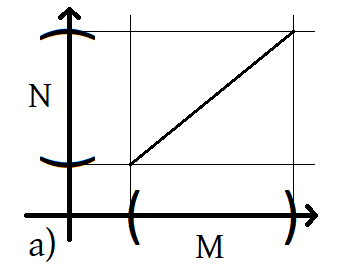
\includegraphics[width=0.4\textwidth,keepaspectratio]{../img/chapter2/surjectiveFunction.png}
            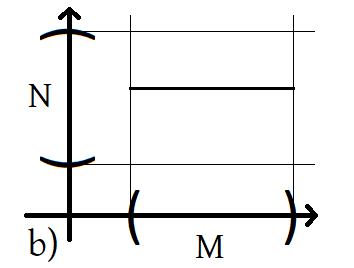
\includegraphics[width=0.4\textwidth,keepaspectratio]{../img/chapter2/surjectiveFunctionNOT.png}
            \caption{Funkce a) je na, funkce b) není.}
        \end{center}
    \end{figure}\FloatBarrier
    Př.: $\varphi$ není prostá, zobrazuje $\mathbb{R}$ na $[0,+\infty)$
    \begin{alignat}{1}
        \varphi:\mathbb{R}&\rightarrow\mathbb{R} \\
        x&\rightarrow x^2 \\
        \varphi((-1,1))&=[0,1)] \\
        \varphi^{-1}([1,4])&=[-2,-1]\cup[1,2]
    \end{alignat}
\end{definition}

\begin{definition}[name={Vzájemně jednoznačné zobrazení, bijekce , isomorfismus}, label=D-bijection]
    Je-li $f:M\rightarrow N$ \hyperref[D-injection]{prostá} a \hyperref[D-surjection]{na}
    říkáme, že je vzájemně jednoznačná
\end{definition}

Pro \hyperref[D-bijection]{vzájemně jednoznačnou funkci} lze definovat inverzní funkci:
\begin{equation}
    f_{-1}:N\rightarrow M; y\in N\rightarrow \text{jediné }x\in M: f(x)=y
\end{equation}
\[
    \textbf{Pozor!}
    \begin{cases}
        f^{-1} \quad\text{pro každou hodnotu zvlášť, je to množina} \\
        f_{-1} \quad\text{inverzní funkce}
    \end{cases}
\]

\begin{definition}[Restrikce, zúžení]
    Je-li $f:M\rightarrow N$ a $A\subset M$: $f|_A$ nazvu restrikce (zúžení) $f$ na $A$
\end{definition}
\begin{example}
    $\varphi(x)=x^2: \varphi|_{[0,+\infty)}$ zobrazuje $[0,+\infty)$ na $[0,+\infty)$ vzájemně
    jednoznačně. Lze tedy definovat $\varphi_{-1}=(\varphi|_{[0,+\infty)})_{-1}(x)=\sqrt{x}$
\end{example}    
        
\begin{definition}[Složená funkce, superpozice]
    Pro $M,N,K$ množiny a \\ $f:M\rightarrow N; g:N\rightarrow K$ funkce definujeme složenou funkci
    \begin{alignat}{2}
        &g\circ f: M\rightarrow K &&\quad M\xrightarrow{f}N\xrightarrow{g}K \\
        &x\in M \rightarrow \left(g(f(x))\right) &&\quad x\rightarrow f(x)\rightarrow\left(g(f(x))\right)
    \end{alignat}
    Budeme psát: $\varphi :M\rightarrow N$ i když $\varphi(x)$ není definované $\forall x\in M$
\end{definition}

\begin{definition}[Definiční obor a obor hodnot]
    \begin{alignat}{1}
        D(\varphi)&=\left\{x\in M: f(x) \text{ je definovaná}\right\} \\
        H(\varphi)&=f\left\{D(\varphi)\right\}
    \end{alignat}
\end{definition}
\begin{example}
    \begin{equation*}
        x^{-1}: \mathbb{R}\rightarrow\mathbb{R} \quad
            D\left(x^{-1}\right)=\mathbb{R}-\left\{0\right\} \quad
            H\left(x^{-1}\right)=\mathbb{R}-\left\{0\right\}
    \end{equation*}
\end{example}

\begin{definition}[name=Monotónost funkce, label=D-monotonic]
    Nechť $f:\mathbb{R}\rightarrow\mathbb{R}$; $M\subset D(f)$. Řeknu, že $f$
    \[
        \text{je}\left.
        \begin{cases}
            \text{rostoucí} \\
            \text{klesající} \\
            \text{nerostoucí} \\
            \text{neklesající}
        \end{cases}
        \right\} \text{na $M$, pokud }\forall x_1,x_2\in M:x_1<x_2\Rightarrow f(x_1)\left.
        \begin{cases}
            < \\
            > \\
            \geq \\
            \leq
        \end{cases}
        \right\}f(X_2)
    \]
    \begin{figure}[ht!]
        \begin{center}
            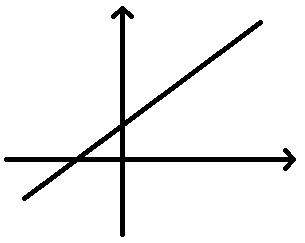
\includegraphics[width=0.24\textwidth,keepaspectratio]{../img/chapter2/monotonic1.png}
            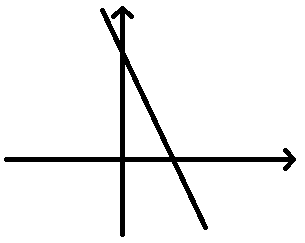
\includegraphics[width=0.24\textwidth,keepaspectratio]{../img/chapter2/monotonic2.png}
            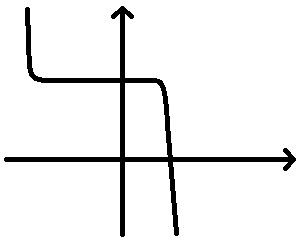
\includegraphics[width=0.24\textwidth,keepaspectratio]{../img/chapter2/monotonic3.png}
            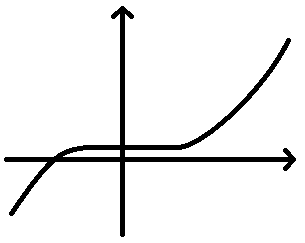
\includegraphics[width=0.24\textwidth,keepaspectratio]{../img/chapter2/monotonic4.png}
            \caption{Ilustrace.}
        \end{center}
    \end{figure}\FloatBarrier
\end{definition}

\begin{definition}[name=Omezenost funkce, label=D-bounded]
    Řekněme, že $f$
    \[
        \text{je}\left.
        \begin{cases}
            \text{omezená shora} \\
            \text{omezená zdola} \\
            \text{omezená}
        \end{cases}
        \right\} \text{na $M$, pokud }\exists K\in\mathbb{R}:\forall x\in M:\left.
        \begin{cases}
            f(x)<K \\
            f(x)>K \\
            \abs{f(x)}<K
        \end{cases}
        \right\}
    \]
\end{definition}

\begin{definition}[name=Symetrie funkce, label=D-symetry]
    Řekněme, že $f$
    \begin{alignat}{1}
        \text{je}\left.
        \begin{cases}
            \text{lichá,} \\
            \text{sudá,} \\
            \text{periodická,}
        \end{cases}
        \right\} \text{pokud}\left.
        \begin{cases}
            \forall x\in D(f) \\
            \forall x\in D(f) \\
            \exists p\in\mathbb{R}:\forall x\in D(f)
        \end{cases}
        \right\} \text{platí} \nonumber\\
        \left.
        \begin{cases}
            -x\in D(f)&\&~f(x)=-f(-x) \\
            -x\in D(f)&\&~f(x)=f(-x) \\
            x+p\in D(f)&\&~f(x)=f(x+p) 
        \end{cases}
        \right\}
    \end{alignat}
\end{definition}

Budeme zkoumat: $f:\mathbb{R}\rightarrow\mathbb{R}$ nebo $f:\mathbb{R}\rightarrow\mathbb{C}$.
Druhou variantu chápeme jako:
\begin{equation}
    f=f_1+if_2;~f_1,f_2:\mathbb{R}\rightarrow\mathbb{R}
\end{equation}

\begin{definition}[name=Okolí, label=D-neighbourhood]
    Nechť $x_0\mathbb{R}, \delta\in(0,\infty)$
    \begin{itemize}
        \item kruhové okolí\quad $U(x_0,\delta):=(x_0-\delta, x_0+\delta)=
            \left\{x\in\mathbb{R}:x_0-\delta<x<x_0+\delta\right\}$ \\
        (v aj \textit{B}: ball)
        \item prstencové okolí\quad $P(x_0,\delta):=U(x_0,\delta)-\left\{x_0\right\}$
        \item pravé kruhové okolí\quad $U_+(x_0,\delta):=\left[x_0,x_0+\delta\right)$
        \item obdobně definujeme \textbf{levé kruhové okolí}, \textbf{pravé prstencové okolí} \\
            a \textbf{levé prstencové okolí}
    \end{itemize}
\end{definition}

Poznámky:
\begin{itemize}
    \item Pro $0<\delta_1<\delta_2\Rightarrow U(x_0,\delta_1)\subset U(x_0,\delta_2)$
    \item Budeme psát: „na jistém $U(x_0)$ platí\dots“, což znamená \\
        $\exists\delta>0:\forall x\in U(x_0,\delta)$ platí\dots
\end{itemize}

\begin{theorem}[name=Hausedorfův princip oddělení, label=T-hausedorf]
    Nechť $x_1,x_2\in\mathbb{R};~ x_1\neq x_2$, pak \\
    $\exists\delta>0$ tak, že $U(x_1,\delta)\cap U(x_2,\delta)=\varnothing$

    Speciálně: $x_1\notin U(x_2,\delta);~x_2\notin U(x_1,\delta)$
\end{theorem}
\begin{proof}
    Volme $\delta=\frac{\abs{x_1-x_2}}{2}$. Tvrdím, že $U(x_1,\delta)\cap U(x_2,\delta)=\varnothing$

    Sporem: ať $\exists y\in U(x_1,\delta)\cap U(x_2,\delta)$, pak
    \begin{gather}
        \abs{x_1-x_2} = \abs{x_1-y+y-x_2}
            \overset{\autoref{T-triangleInequality}}{\leq} \nonumber \\
        \abs{x_1-y}+\abs{y-x_2} < 2\delta = \abs{x_1-x_2}
    \end{gather}
    Tedy $\abs{x_1-x_2} < \abs{x_1-x_2}$, což je spor.
\end{proof}

\begin{definition}[name=Limita, label=D-limit]
    Nechť $x_0\in\mathbb{R}$ a $f$ je fce def na jistém $P(x_0)$

    Číslo $A\in\mathbb{R}$ nazvu limitou $f$ v $x_0$, pokud
    \begin{equation}\label{D-limit-215}
        \forall\epsilon>0~\exists\delta>0: x\in P(x_0,\delta) \Rightarrow f(x)\in U(A,\epsilon)
    \end{equation}
    
    Značení:
    \begin{itemize}
        \item $\lim_{x\to x_0}f(x)=A$
        \item $f(x)\rightarrow A$ pro $x\rightarrow x_0$
    \end{itemize}
\end{definition}

Terminologie: pokud existuje $\lim_{x \to x_0}f(x)\in\mathbb{R}$ říkáme, že $f$
má vlastní limitu ve vlastním bodě

Poznámky:
\begin{itemize}
    \item Limita závisí na $f$ v okolí $x_0$
    \item Jiné zápisy \autoref{D-limit-215}
        \begin{alignat}{1}
            \forall\epsilon>0~\exists\delta>0&:f(P(x_0,\delta))\subset U(A,\epsilon) \\
            \forall\epsilon>0~\exists\delta>0&:\forall x\in\mathbb{R}:
                \left[0<\abs{x-x_0}<\delta \Rightarrow\abs{f(x)-A}<\epsilon\right]
        \end{alignat}
\end{itemize}

\begin{theoremAlph}[Jednoznačnost limity]
    Buď $\lim_{x \to x_0}f(x)=A$ a $\lim_{x \to x_0}f(x)=B$
    
    Pak $A=B$
\end{theoremAlph}
\begin{proof}
    Sporem: ať $A\neq B$
    \begin{alignat}{1}
        \text{\autoref{T-hausedorf}}&\quad \exists\epsilon>0:
            U(A,\epsilon)\cap U(B,\epsilon)=\varnothing \\
        \text{\autoref{D-limit-215} pro $A$}&\quad \exists\delta_1>0:x\in P(x_0,\delta_1)
            \Rightarrow f(x)\in U(A,\epsilon) \\
        \text{\autoref{D-limit-215} pro $B$}&\quad \exists\delta_2>0:x\in P(x_0,\delta_2)
            \Rightarrow f(x)\in U(B,\epsilon) \\
        \text{Definujme }&\quad \delta=min(\delta_1,\delta_1) \\
        \text{Odvodíme spor }&\quad \forall x\in U(x_0,\delta):f(x)\in
            U(A,\epsilon)\cap U(B,\epsilon)=\varnothing
    \end{alignat}
\end{proof}

\begin{example}
    \begin{alignat}{1}
        &\lim_{x\to 2}x^2=4 \\
        \text{cíl:}\quad& \forall\epsilon>0~\exists\delta>0:x\in P(2,\delta)
            \Rightarrow f(x)\in U(4,\epsilon) \\
        \text{fix $\epsilon>0$}\quad& \text{hledám $\delta>0$} \\
        \text{chci:}\quad& 4-\epsilon<x^2<4+\epsilon \\
        \text{lze předpokládat, }& \text{že $\epsilon<1$, protože pokud $\epsilon\geq 1$,
            pak $U(4,\frac{1}{2})\subset U(4,\epsilon)$} \\
        \text{vidíme:}\quad& \sqrt{4-\epsilon}<x<\sqrt{4+\epsilon} \\
        \text{volme:}\quad& \delta=min(2-\sqrt{4-\epsilon}, \sqrt{4+\epsilon}-2) \\
        \text{volme:}\quad& x\in P(2,\delta) \\
        \text{chci dokázat, }& \text{že platí cíl: }f(x)\in U(4,\epsilon) \\
        \text{odhad shora:}\quad& x^2-4\leq(2+\delta)^2-4=4+4\delta+\delta^2-4=(4+\delta)\delta \\
        & \leq(4+\sqrt{4+\epsilon}-2)(\sqrt{4+\epsilon}-2) \\
        & =(\sqrt{4+\epsilon}+2)(\sqrt{4+\epsilon}-2)=4+\epsilon-4=\epsilon \\
        \text{odhad odspodu:}\quad& x^2-4\geq(2-\delta)^2-4=4-4\delta+\delta^2-4=\delta(\delta-4) \\
        & \dots\text{zbytek obdobně}
    \end{alignat}
\end{example}

\begin{definition}[Jednostranné limity]
    Nechť $x_0\in\mathbb{R}$, $f$ definovaná na jistém $P_+(x_0)$ (resp. $P_-(x_0)$). Pak
    číslo $A$ nazvu limitou $f$ v bodě $x_0$ zprava (zleva), pokud:
    \begin{equation}
        \forall\epsilon>0~\exists\delta>0:\forall x\in P_{+(-)}(x_0,\delta):f(x)\in U(A,\epsilon)
    \end{equation}

    Značení (zleva obdobně):
    \begin{itemize}
        \item $\lim_{x\to x_0+}f(x)=A$
        \item $f(x)\rightarrow A$ pro $x\rightarrow x_0+$
    \end{itemize}
\end{definition}

\begin{example}
    \begin{alignat}{1}
        \lim_{x\to 0+}sgn(x)&=1 \\
        \lim_{x\to 0-}sgn(x)&=-1
    \end{alignat}
\end{example}

\begin{theorem}[Jednostranné vs oboustranná limita]
    Buď $x_0\in\mathbb{R}$, $f$ definovaná na jistém $P(x_0,\delta)$, pak následující
    tvrzení jsou ekvivalentní
    \begin{alignat}{1}
        \lim_{x\to x_0}&=A \label{T-1v2limit-241}\\
        \lim_{x\to x_0+}&=A \land \lim_{x\to x_0-}=A \label{T-1v2limit-242}
    \end{alignat}
\end{theorem}
\begin{proof}
    \autoref{T-1v2limit-241} $\Rightarrow$ \autoref{T-1v2limit-242} triviální
    
    \autoref{T-1v2limit-242} $\Rightarrow$ \autoref{T-1v2limit-241} volme $\epsilon>0$,
    podle \autoref{T-1v2limit-242}
    \begin{gather}
        \exists\delta_1>0:\forall x\in P_+(x_0,\delta_1):f(x)\in U(A,\epsilon) \\
        \exists\delta_2>0:\forall x\in P_-(x_0,\delta_1):f(x)\in U(A,\epsilon)
    \end{gather}
    volme $\delta=min(\delta_1, \delta_2)$ (protože
    $P(x_0,\delta)\subset P(x_0,\delta_1)\cup P(x_0,\delta_2)$)
    
    Potom $P(x_0,\delta):f(x)\in U(A,\epsilon)$
\end{proof}
\begin{example}
    Neexistuje $\lim_{x\to 0}sgn(x)$
\end{example}

\begin{theoremAlph}[name=Ekvivalentní limity, label=T-equivalentLimits]
    Buď $x_0\in\mathbb{R}$, $f$ definovaná na jistém $P(x_0)$. Pak
    \begin{equation}
        \lim_{x\to x_0}f(x)=A \Leftrightarrow \lim_{x\to x_0}f(x)-A=0
            \Leftrightarrow \lim_{x\to x_0}\abs{f(x)-A}=0
    \end{equation}
\end{theoremAlph}
\begin{proof}
    \begin{gather}
        \forall\epsilon>0~\exists\delta>0:\forall x\in P(x_0,\delta):\abs{f(x)-A}<\epsilon \\
        \abs{f(x)-A}<\epsilon \Leftrightarrow f(x)\in U(A,\epsilon)
    \end{gather}
\end{proof}

\begin{lemma}[name=Chování funkce v okolí limity, label=L-limitNeighbourhood]\noindent
    \begin{enumerate}
        \item Nechť $f$ má v $x_0\in\mathbb{R}$ limitu $A\in\mathbb{R}$. Pak existuje
            $P(x_0)$ takové, že $f$ je na $P(x_0)$ omezená. Tj.
            \begin{equation}\label{L-limitNeighbourhood-247}
                \exists\delta>0\exists K>0:\forall x\in P(x_O,\delta): \abs{f(x)}<K
            \end{equation}
        \item Nechť $f$ má v $x_0\in\mathbb{R}$ limitu $A\neq 0$, pak
            \begin{equation}\label{L-limitNeighbourhood-248}
                \exists\Delta>0\exists\delta>0:\forall x\in P(x_O,\delta): \abs{f(x)}>\Delta
            \end{equation}
    \end{enumerate}
\end{lemma}
\begin{proof}\noindent
    \begin{enumerate}
        \item Volme $\epsilon=1$ v definici limity. Pak
            \begin{equation}
                \exists\delta>0:\forall x\in P(x_0,\delta): A-1<f(x)<A+1
            \end{equation}
            tj. $f(x)\in U(x_0,\delta)$. Stačí volit $K=max(\abs{A-1},\abs{A+1})$. pak
            \begin{equation}
                \forall x\in P(x_0,\delta):-K<leq A-1<f(x)<A+1\leq K
            \end{equation}
        \item $A\neq 0$, předpokládejme $A>0$ ($A<0$ podobně)
        \begin{gather}
            \begin{alignat}{1}
                \text{dle \autoref{T-hausedorf}} &\quad\exists\epsilon>0:
                    U(A,\epsilon)\cap U(0,\epsilon)=\varnothing \\
                \text{z \autoref{D-limit}} &\quad\exists\delta>0:
                    \forall x\in P(x_0,\delta):f(x)\in U(A,\epsilon) \\
                \text{máme $\delta>0$ a volíme } &\quad\Delta=\epsilon/2 
            \end{alignat}\\
            \forall x\in P(x_0,\delta):f(x)\in U(A,\epsilon) \\
            U(A,\epsilon)\cap U(0,\epsilon)=\varnothing \\
            \abs{f(x)-0}\geq\epsilon>\Delta
        \end{gather}    
    \end{enumerate}
\end{proof}

\begin{lemma}[name=Limita součinu, label=T-limitMultiplication]
    Buďte $f$, $g$ definované na jistém $P(x_0)$, $f$ omezená na $P(x_0)$ a
    $\lim_{x\to x_0}g(x)=0$. Pak
    \begin{equation}
        \lim_{x\to x_0}f(x)g(x)=0
    \end{equation}
\end{lemma}
\begin{proof}
    Volme $\epsilon>0$ libovolné. Vím
    \begin{alignat}{1}
        \exists\delta_1>0,K>0: &\forall x\in P(x_0,\delta_1): \abs{f(X)}<K 
            \label{T-limitMultiplication-P-258} \\
        \exists\delta_2>0: &\forall x\in P(x_0,\delta_2): \abs{g(X)}<\epsilon/K
            \label{T-limitMultiplication-P-259}
    \end{alignat}
    Chci součin odhadnout epsilonem
    \begin{equation}
        \abs{f(x)g(x)}<K\abs{g(x)}<\epsilon
    \end{equation}
    Volme $\delta=min(\delta_1,\delta_2)$. Potom platí
    \begin{equation}
        \forall x\in P(x_0,\delta):
            \abs{f(x)g(x)}\overset{\autoref{T-limitMultiplication-P-258}}{<}
            K\abs{g(x)}\overset{\autoref{T-limitMultiplication-P-259}}{<}K\frac{\epsilon}{K}
            =\epsilon
    \end{equation}
    Tzn. $f(x)g(x)\in U(0,\epsilon)$
\end{proof}
\begin{example}\noindent
    \begin{enumerate}
        \item $\lim_{x\to 0}sgn(x)x^2=0$, protože $\lim_{x\to 0}x^2=0$ (z definice)
            a $\abs{sgn(x)}\leq 1$.
            
            Pozor: $\lim_{x\to 0}sgn(x)$ neexistuje!
        \item $\lim_{x\to 0}x~sin(1/x)=0$ 
    \end{enumerate}
    \begin{figure}[ht!]
        \begin{center}
            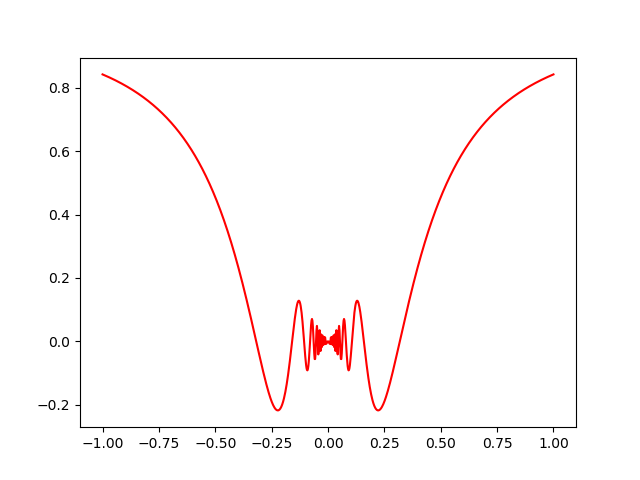
\includegraphics[width=0.4\textwidth,keepaspectratio]{../img/chapter2/limitMultiplication.png}
            \caption{Graph of the function $x~sin(1/x)$.}
        \end{center}
    \end{figure}\FloatBarrier
\end{example}

\begin{theorem}[name=Aritmetika limit, label=T-limitArithmetic]
    Nechť $x_0\in\mathbb{R}$, $A,B\in\mathbb{R}:$ $\lim_{x\to x_0}f(x)=A$,
    $\lim_{x\to x_0}g(x)=B$. Pak platí
    \begin{alignat}{1}
        \lim_{x\to x_0}\left(f(x)\pm g(x)\right) &= A\pm B \label{T-limitArithmetic-addition} \\
        \lim_{x\to x_0}\left(f(x)g(x)\right) &= AB \label{T-limitArithmetic-multiplication} \\
        \text{je-li navíc $B\neq 0$ }\quad \lim_{x\to x_0}\left(\frac{f(x)}{g(x)}\right)
            &= \frac{A}{B} \label{T-limitArithmetic-division}
    \end{alignat}
\end{theorem}
\begin{proof}\noindent
    \begin{enumerate}
        \item \autoref{T-limitArithmetic-addition} pro $\oplus$ ($\ominus$ obdobně).
        
            Chceme
            \begin{equation}
                \forall\epsilon>0\exists\delta>0: \forall x\in P(x_0,\delta):
                    f(x)+g(x)\in U(A+B,\epsilon)
            \end{equation}
            Víme
            \begin{alignat}{4}
                &\forall\epsilon'>0&\exists\delta'>0: &\forall x\in P(x_0,\delta'):
                    ~&f(x)\in U(A,\epsilon') \label{T-limitArithmetic-P-266} \\
                &\forall\epsilon''>0&\exists\delta''>0: &\forall x\in P(x_0,\delta''):
                    ~&g(x)\in U(B,\epsilon'') \label{T-limitArithmetic-P-267}
            \end{alignat}
            Předběžně
            \begin{equation}
                \abs{f(x)+g(x)-A-B} \overset{\autoref{T-triangleInequality}}{\leq}
                    \abs{f(x)-A} + \abs{g(x)-B}
            \end{equation}
            Fix $\epsilon>0$ libovolné.
            
            Z \autoref{T-limitArithmetic-P-266} s $\epsilon'=\epsilon/2$ dostanu $\delta'>0$
            (takové, že platí zbytek \autoref{T-limitArithmetic-P-266})
            
            Z \autoref{T-limitArithmetic-P-267} s $\epsilon''=\epsilon/2$ dostanu $\delta''>0$
            
            Definujme $\delta=min(\delta',\delta'')$ (aby pro $\delta$ platily obe rovnice). Pak
            \begin{equation}
                \forall x\in P(x_0,\delta)\subset P(x_0,\delta')\cap P(x_0,\delta''):
                    f(x)+g(x)\in U(A+B,\epsilon)
            \end{equation}
        \item Chci $f(x)g(x)-AB\rightarrow 0$ pro $x\rightarrow x_0$
            \begin{equation}
                f(x)g(x)\pm f(x)B-AB = f(x)(g(x)-B) + (f(x)-A)B
            \end{equation}
            \begin{itemize}
                \item $f(x)$ je omezená na jistém $P(x_0)$ podle \autoref{L-limitNeighbourhood}
                \item $(g(x)-B)\rightarrow 0$ podle \autoref{T-equivalentLimits}
                \item $f(x)(g(x)-B)\rightarrow 0$ podle \autoref{T-limitMultiplication}
                    a prvních dvou bodů
                \item obdobně $(f(x)-A)B\rightarrow 0$ (konstanta $B$ je omezená funkce)
                \item a tedy celá pravá strana $\rightarrow 0$ podle
                    \autoref*{T-limitArithmetic}-\autoref{T-limitArithmetic-addition}
            \end{itemize}
        \item Ukážu
    \end{enumerate}
\end{proof}
